\documentclass[english, 11pt]{article}

\usepackage{amsmath, amssymb, bm}
\usepackage{blindtext}
\usepackage{graphicx}
\usepackage[utf8]{inputenc}
\usepackage{comment}
\usepackage[paperwidth=8.5in, paperheight=11in]{geometry}
\usepackage{color}
\usepackage{enumitem}
\usepackage{babel,blindtext}
\usepackage{caption}

\graphicspath{ {Desktop/} }
\title{\textbf{CPSC 490 Final Paper: Synthesizing DSP Filters on Non-Commutative Sound Samples}}
\author{Kate Rogers\\ \textit{Advised by Professor Ruzica Piskac}}
\date{\today}
\begin{document}
\maketitle

\section{Introduction}

The great proliferation of computer music programming languages points to the difficulty of building a natural interface for users who want to computationally interact with musical data. Programming applications in the domain of computer music, and specifically digital signal processing (DSP), requires that users not only grasp fundamental programming techniques, but also have a large domain specific knowledge on time and signal manipulations. The amount of prerequisite skill and effort to overcome these barriers is often higher than many users are able to commit.  \\ \\
Furthermore, the difficulty of programming DSP applications is often not commensurate with the creative intentions. As a motivating example, imagine a user was to reconstruct the filter that was used to transform an audio clip. In this case the user has the original audio file, and the transformed audio file, but does not know how this transformation happened. In the standard approach, a user would need to be a domain expert and listen to the two files, and aurally estimate which kinds of filters were used to achieve the transformation. Once the user has some suspicion as to the appropriate filter types that will be needed, the user must write a program in some language (SuperCollider~\cite{supercollider}, etc) that implements the DSP filter the user has in mind. Further still, the user will then need to spend time tweaking the filter parameters to find the best fit. 

\section{DSP-PBE}

To simplify the user process, we introduce DSP programming by example (DSP-PBE). With DSP-PBE, the user simply provides our tool with the original audio (input), and the transformed audio (output), and it will automatically receive a DSP filter that approximates the transformation. \\ \\
As an example, this was the approach used for the audio files in Figure 1. In this example, a user provided a clip of a 'cartoon spring' in Figure 1a, and the same sound as it had been transformed with a lowpass filter at 800 Hz as shown in Figure 1b. However the nature of the transformation is unknown to the user and they wish to discover the filter needed. Our DSP-PBE tool is able to synthesize a lowpass filter at 947 Hz, that when applied to the original sound, produces the waveform shown in Figure 1c. While the solution is not exact, the difference is not significantly noticeable to an untrained ear.
\begin{figure}[!htb]
\minipage{0.32\textwidth}
  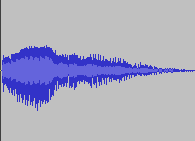
\includegraphics[width=\linewidth]{original.png}
  \caption*{(a) Input Example}\label{fig:image1}
\endminipage\hfill
\minipage{0.32\textwidth}
  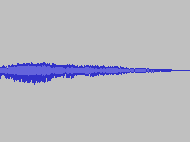
\includegraphics[width=\linewidth]{lpf800.png}
  \caption*{(b) Output Example}\label{fig:image2}
\endminipage\hfill
\minipage{0.32\textwidth}%
  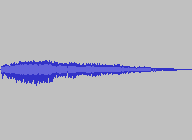
\includegraphics[width=\linewidth]{lpf950.png}
  \caption*{(c) Generated}\label{fig:image3}
\endminipage
\caption{The waveforms (a) and (b) are provided as examples, and DSP-PBE synthesizes a filter that produces (c)}
\end{figure}
\subsection{DSP-PBE: The Problem}
The problem of DSP programming by example is formally defined as follows: Given an input waveform \texttt{$I$} and an output waveform \texttt{$O$}, construct a DSP filter \texttt{$F$}, to minimize the aural distance \texttt{dist} between the \texttt{$O$} and \texttt{$F(I)$}. In a single line: \\

\centerline{ \texttt{Find $F$ such that dist$(O, F(I))$ = $0$}} ~\\
The two key components of this statement are the definition of distance \texttt{(dist)} and a search technique to find \texttt{$F$}. A distance metric that is faithful to the psycho-acoustics of the human ear is critical for a useful tool.  \\ \\
\begin{comment} 
As an example, taking a trivial distance function that returns the difference in length of the two audio samples will allow a delay filter to satisfy any example pair of samples.
\end{comment}
Additionally, an efficient search algorithm is critical, as the space of possible DSP filters is very large. Not only do we need to consider a wide variety of filters, we need to consider the space of parameters for each filter, as well as the different ways of combining multiple filters.


\begin{comment} 
Currently, Ruzica Piskac and her team have a DSP-PBE Synthesizer that works on commutative sound samples. The distance calculation they used will remain constant for the terms of my project. My task is to figure out how to apply their work to non-commutative sound samples by altering/designing the search algorithm used.
\end{comment}

\section{Background Information}

\subsection{The Sound Sample}

The sound sample is originally a waveform graph. A waveform graph is a way of storing an audio bitstream on a computer. This wav file can be represented as a graph where the x-axis represents time and the y-axis represents amplitude, or similarly, how much charge one puts on a membrane of a speaker to produce sound waves. This waveform graph is represented in the time domain. An example of a waveform is seen in the figure below:
\begin{figure}[!htb]
\includegraphics[width=\textwidth]{Sound_Sample} 
\caption{Graph of a sound sample of a coyote howl.}\label{fig:image4}
\end{figure} \\
A second way of representing the sound sample is through the spectrogram of the waveform. This is a graph whose x-axis is frequency and whose y-axis is amplitude or how loud the sound sample is at that frequency. It is common to see many large spikes at certain frequencies. We use this form of the sound sample to help us recreate the output filter using DSP-PBE. The spectrogram of the waveform is in the frequency domain and is the result of the FFT operation. An example of a spectrogram of the waveform can be seen below:
\begin{figure}[!htb]
\centerline{\includegraphics[scale = 0.45]{Spectrum_Graph}} 
\caption{Spectrogram of the sound sample of a coyote howl.}\label{fig:image5}
\end{figure}\\ \\
The transition between the time domain (waveform) and the frequency domain (spectrogram) will be key to solving the DSP-PBE problem.

\subsection{Filters}

Currently, the DSP-PBE Synthesizer works with two filters, highpass and lowpass. All filters can be written as equations, so for the filters we are using, the equations will be given as well. In all filters, x is the input signal and y is the output signal. The information in brackets after the x or y is the index of the sample, as all sound samples are indexed. The $a_i$ is called a filter coefficient. Filter coefficients contain values from 0 to 1. The coefficient with a subscript 0 indicates a non-delayed signal, while the coefficient with a subscript 1 indicates a signal with a one-sample delay, etc. These values affect the frequency response of the filters.

\subsubsection{Lowpass Filter}

A lowpass filter is a filter that attenuates high frequencies. In other words, it diminishes the effect of high frequencies, making the low frequencies more prominent. \\

\textbf{Equation:}

\texttt{$y[n]$ = ($a_0$ * $x[n]$) + ($a_1$ * $x[n-1]$) + ... + ($a_i$ * $x[n-i]$)}
\par Where \texttt{$i$} represents the index of the last stored sample.

\subsubsection{Highpass Filter}

A highpass filter is a filter that attenuates low frequencies. In other words, it makes the high frequencies even more prominent than they already are. \\ 

\textbf{Equation:}

\texttt{$y[n]$ = ($a_0$ * $x[n]$) - ($a_1$ * $x[n-1]$) - ... - ($a_i$ * $x[n-i]$)}
\par Where \texttt{$i$} represents the index of the last stored sample. \\ \\ 
A high pass filter is basically the opposite of a lowpass filter as the equations are the same except addition symbols in low pass filters are traded out for subtraction symbols in high pass filters. \\ \\
These equations for these filters represent functions in the time domain. However, when we use the aural distance function, we must transform the sound sample to the frequency domain. This transformation will be described in the following section.

\begin{comment}
\subsubsection{White Noise}
\textbf{Last thing that we do, will check back once I'm done with refinement types for others} \\
White noise is a random signal with equal intensities at different frequencies. What does white noise do to sample? Mask it? \\

\textbf{Equation:}
\texttt{$y[n]$ = ($a_0$ * $x[n]$) + random (1 - $a_0$)}
\par Where random is a random number from ? to ? to represent ?. \\ \\
Also, shouldn't there not be a refinement type for it? Aren't we just adding it to a high pass or low pass filter to get some variance in the filter?
\end{comment}

\subsection{Sound Resynthesis}

Sound resynthesis has a similar high level goal to DSP-PBE in that it works to recreate a sound sample. However, it can be thought of as half of DSP-PBE in that it only takes an output sound file, not an input. Basically, given an audio clip, sound resynthesis will build a synthesizer that will produce that sound by adding together sine waves~\cite{resynthesis}. Although sound resynthesis is not exactly like DSP-PBE, we can use this technique to better understand the workings of a sound wave.

\section{Aural Distance}

As a distance metric, we used as a starting point the literature on acoustic fingerprinting~\cite{fingerprinting}. Acoustic fingerprinting is the concept of creating a condensed, distinct summary of an audio file that can be used later to identify that audio file or to look it up in a database. Acoustic fingerprints represent how the file will sound to the human ear regardless of how it is represented in a digital format. There are numerous ways to develop acoustic fingerprints and companies like Shazam and Sound-Hound have developed complex algorithms to create accurate fingerprints even from low quality files recorded on a cellphone mic. One of Shazam's engineers released a paper detailing their process several years ago~\cite{Shazam}. We used this paper as an inspiration for our checker. The Shazam method uses Fast Fourier Transforms to convert the WAVE file into a spectrogram plotted over time. Then they plot the (frequency, time) coordinates with the greatest amplitude to create a star map of points that become the files audio fingerprint. We use a similar strategy by first performing a real Fast Fourier Transform on the imported WAVE file and then picking out the frequency peaks in each time frame. \\ \\
Fast Fourier Transforms are the key to a good acoustic fingerprint. In order to complete this project, we were able to find several Haskell libraries that provide DFT and FFT functions but the majority of our reading on this topic was on how to interpret the results of these functions. The results of these functions are not presented in an intuitive manner and one must take into account negative frequencies. The return arrays are presented with the zero frequency component or DC, followed by positive frequencies up until the Nyquist frequency (sampling frequency divided by 2) after which all the elements represent negative frequencies which are irrelevant to a spectrogram. For this reason, we had to adjust the checker to only observe the array elements from to the Nyquist frequency and exclude the zeroth element and all the negative frequency. \\ \\
In our readings about the results of FFT, we came across the topic of spectral leakage. Frequency and time are continuous spectra. FFT, however, relies on a discrete representation of the sound wave over time and therefore returns a discrete representation of the frequency spectrum. Each return element is a frequency ``bin'', and depending on the scale of your return array the size of this bins varies. In order for each bin to correspond to 1 Hz the size of the return vector must be equal to the sampling frequency (44,100 Hz). If each bin is not 1 Hz, the effects of spectral leakage will be seen. This occurs when the bins do not correspond to the exact frequency peaks of the sound. The amplitude from the peaks that fall in between bins will ``leak'' over into the closest bin and create a distorted spectrogram. For this reason we had to adjust the size of the FFT return arrays to be 44,100. Although this slows down the process of FFT, it provides the most accurate representation of the sound and for our purposes frequency accuracy is paramount. \\ \\
This idea helped us to create the \texttt{dist} function that we will use to measure aural distance and be faithful to the psycho-acoustics of the human ear. Obviously, the goal will be to have the \texttt{dist$(O, F(I))$ = 0}. But, the DSP-PBE Synthesizer can only get us so close to this metric. We have provided a default threshold distance for the aural distance. This was obtained by testing samples that we thought were close enough to each other and obtaining the aural distance metric on those. The threshold distance can be changed by the user depending on their needs or requirements. This part (the distance funtion) had already been completed by the team in prior work, so the main focus of this paper will be around the Search Algorithm, which will take advantage of this idea of aural distance to check the accuracy of the DSP-PBE checker and search algorithm.

\section{Search Algorithm}

Because the search space of possible programs is extremely large, search procedures must be exceptionally efficient. A couple options are listed below.

\subsection{Gradient Descent}

Gradient descent could be a viable search technique. It is the current search process used in our prototype. However, one trouble with this approach is that we have lots of local minimums in the space of optimization. Let's take the example of trying to learn a low-pass filter threshold frequency. If our initial threshold frequency is too low (cutting off too much), and just on the other side of the frequency we need, SGD will easily send us in that direction. However, if the spectrogram of waveform has a frequency spectrum that is mostly inactive, SGD will detect a plateau and tell us we have found a global minimum, when in fact we are stuck at a local minimum. So, in order to overcome this problem, we can add additional techniques to the search algorithm to help us find a filter.

\subsection{Refinement Types}

Refinement types are a way of giving an abstract description of the behavior of a function. \\ \\
For example, we can describe the function \\ \\
\centerline{\texttt{map::[a]} $\,\to\,$ \texttt{[b]},}\\ \\
that captures some properties of the behavior of the function, \\ \\
\centerline{\texttt{f::xs:[a]} $\,\to\,$ \texttt{ys:[b]} \textbar \texttt{ length xs == length ys},} \\ \\
in this case that the length of the lists are still equal. In a similar style for DSP, we can write predicates about the filters available to us during synthesis. For example, a low-pass filter could be described as the refinement type that says the amplitude of the frequencies greater than the threshold frequency have decreased in the output Audio. \\ \\
\centerline{ \texttt{lpf::t:Float} $\,\to\,$  \texttt{xs:Audio} $\,\to\,$ \texttt{ys:Audio} \textbar}
\centerline{\texttt{ ($\forall$$f_1$ $\in$ spectrogram(xs)}, \texttt{ $\forall$$f_2$ $\in$ spectrogram(ys))}: } \centerline{\texttt{(}$f_1$ $\textgreater$ \texttt{t}  $\land$  $f_2$ $\textgreater$ \texttt{t}  $\land$  $f_1$ == $f_2$ $\implies$ \texttt{(amp($f_1$) $\textgreater$ amp($f_2$))}} ~\\
Where \texttt{t} represents the level at which the lowpass filter is applied, \texttt{spectrogram} represents the spectrogram of the sound sample, $f_i$ represents a frequency, and \texttt{amp()} represents the amplitude of the frequency. This refinement type can be abbreviated into \texttt{$r_{lpf}$(t, xs, ys)}, a predicate on a threshold frequency \texttt{t} and the two audio files \texttt{xs, ys}. \\ \\
Additionally, a high-pass filter could be described as the refinement type that says the amplitude of the frequencies less than the threshold frequency have decreased in the output Audio. \\

\centerline{ \texttt{hpf::t:Float} $\,\to\,$  \texttt{xs:Audio} $\,\to\,$ \texttt{ys:Audio} \textbar }
\centerline{\texttt{ ($\forall$$f_1$ $\in$ spectrogram(xs)}, \texttt{ $\forall$$f_2$ $\in$ spectrogram(ys))}: } \centerline{($f_1$ $\textless$ \texttt{t}  $\land$  $f_2$ $\textless$ \texttt{t}  $\land$  $f_1$ == $f_2$ $\implies$ \texttt{(amp($f_1$) $\textgreater$ amp($f_2$))}} ~\\
Where \texttt{t} represents the level at which the highpass filter is applied, \texttt{spectrogram} represents the spectrogram of the sound sample, $f_i$ represents a frequency, and \texttt{amp()} represents the amplitude of the frequency. This refinement type can be abbreviated into \texttt{$r_{hpf}$(t, xs, ys)}, a predicate on a threshold frequency \texttt{t} and the two audio files \texttt{xs, ys}.

\subsection{Combination of Search Algorithms}

One hypothesis as to how we would combine both algorithms would be through a feedback loop. We will use the refinement types to select a filter with a parameter. We then send that information into gradient descent to find a more precise filter representation (more accurate parameter measure). We will then apply this filter with the new parameter value from gradient descent to the input sound sample. Next, we will send this new sound sample $(F(I))$ and the original output sound sample $(O)$ to the aural distance function \texttt{dist}. If the \texttt{dist} function returns a value lower than the threshold distance given by us or the user, then we will accept that filter and return it to the user. If it is not, we will attempt to refine our parameter for the filter. An example of this can be seen in the diagram below: 
\begin{figure}[!htb]
\centerline{\includegraphics[width=\textwidth]{CPSC2}}
\caption{Flow diagram of the DSP-PBE Synthesizer}\label{fig:image6}
\end{figure}\\ 
This loop could become more complicated as multiple filters could be applied to one sound sample once the parameter has been tuned to the best value. This idea will be discussed later in this paper.

\subsubsection{Filter List}

For the DSP-PBE problem on sound samples, we will have a list of filters and corresponding refinement types. The goal for the filter list is to have enough variance in the filters in the list so that gradient descent can then refine the parameter for the filter (finding the global minimum and not getting caught at a local minimum), and no one value of the filter parameter will be overlooked. However, we are going to have to strike a balance between accuracy and length of filter list because the longer the filter list is, the longer it will take to search through all of the filters and corresponding refinement types. As an example, a filter list with only low pass filters would look as below:

\begin{enumerate}
{\setlength\itemindent{150pt} \item{\texttt{lpf($\delta$, xs, ys)}}}
{\setlength\itemindent{150pt} \item{\texttt{lpf(2$\delta$, xs, ys)}}}
\end{enumerate}
\centerline{\bm{$\vdots$}} ~\\
Where $\delta$ is the smallest variance necessary for gradient descent to find the global minimum from this delta and not a local minimum, and the largest variance necessary so any two filters would not overlap. This delta will need to be discovered by practice. 

\subsubsection{Ordering of Refinement Types}

As stated above, the longer the filter list becomes, the longer it will take to search through the list to find a refinement type that holds with the spectrogram of the input and output sound samples. In order to combat this, we could order the filters accordingly, to decrease the time it takes to search through them. We could also attempt to increase the accuracy of the parameters for the filters we know hold on our sound samples. \\ \\
Let's take our filter list created above. For some $\delta$ not yet discovered, a filter list with only lowpass filters will look as follows:

\begin{enumerate}
{\setlength\itemindent{137pt} \item{\texttt{lpf($\delta$, xs, ys)}}}
{\setlength\itemindent{137pt} \item{\texttt{lpf(2$\delta$, xs, ys)}}}
\end{enumerate}
\centerline{\bm{$\vdots$}} 
\begin{enumerate}[resume]
{\setlength\itemindent{137pt} \item{\texttt{lpf(maxf - 2$\delta$, xs, ys)}}}
{\setlength\itemindent{137pt} \item{\texttt{lpf(maxf - $\delta$, xs, ys)}}}
\end{enumerate}
As stated above, we know a low-pass filter could be described by a refinement type stating that the amplitude of the frequencies greater than the threshold frequency value have decreased in the output Audio. For this reason, we know that if any lowpass filter is applied in our output sound sample, the refinement type with the greatest threshold frequency in our filter list will hold for our input and output spectrograms (in this case \texttt{lpf(maxf - $\delta$, xs, ys)}). Formally, we know: \\ \\
\centerline{\texttt{xs::Audio $\land$ ys::Audio $\land$ $r_{lpf}$(t, xs, ys) $\implies$}} \\
\centerline{\texttt{ $\forall$ t' $\textgreater$ t. $r_{lpf}$(t', xs, ys)}} ~\\
So, to attempt to decrease the number of filters tried, we could test the greatest threshold frequency lowpass filter in the filter list, and if it does not hold, we can skip all other lowpass filters in the list. The opposite would hold true for highpass filters: \\ \\
\centerline{\texttt{xs::Audio $\land$ ys::Audio $\land$ $r_{hpf}$(t, xs, ys) $\implies$}}\\
\centerline{\texttt{ $\forall$ t' $\textless$ t. $r_{hpf}$(t', xs, ys)}} ~\\
As we create more refinement types for other filters, we can create different orders to decrease the number of refinement types needed to test to find one that hold for our input and output spectrograms. \\ \\
If we want to increase the accuracy for our refinement types, the order for the filter list will need to be different. If we look at the example filter list above, we would want to start from the lowest threshold frequency filter in the list (\texttt{lpf($\delta$, xs, ys)}) and increase the threshold frequency level from there. This way, we won't skip over our threshold frequency at any point (and therefore end up with a local minimum in gradient descent rather than the global minimum). For highpass filters, we would again want to do the opposite of the lowpass filters and start with the highest threshold frequency value available and decrease that value when searching for the optimal threshold frequency level. Again, we would hopefully be able to make these optimizations with other filter/refinement type additions. This will be the easiest way to increase accuracy or decrease time (or a combination of both) to optimize our DSP-PBE tool.

\subsubsection{Application of Refinement Types}

Given our ordered filter list, we can update our flow chart from Figure~\ref{fig:image6}. The choice of a filter will depend on the order described in the previous section. First, we check the worst case scenario for each filter type. If the worst case scenario for one filter holds, then we go back and test the filters in the order that will correctly increase accuracy for that filter. Otherwise, we skip that filter type all together and move on to the next one. The flow chart below describes the choice of a refinement type from the filter list:
\begin{figure}[!htb]
\centerline{\includegraphics[scale = 0.55]{CPSC490FlowFLChoose}}
\caption{Flow diagram of refinement type choice}\label{fig:image7}
\end{figure}\\ 
Only after finding the correct refinement type parameter will we send that filter corresponding to it to gradient descent to further optimize the parameter. Finally, we check the aural distance of the filter on the input sound sample ($F(I)$) and the output sound sample ($O$), and complete the feedback loop according to the results. The updated flow chart is below:
\begin{figure}[!htb]
\centerline{\includegraphics[width=\textwidth]{CPSC}}
\caption{Flow diagram of DSP-PBE Synthesizer with filter list}\label{fig:image8}
\end{figure}

\begin{comment}
Once an order has been found that best optimizes the refinement type list, we then need to apply the refinement types. In order to apply the refinement type, we will go through our refinement type list and test each if each one holds true on the spectrogram of the input and output sound samples, skipping the ones accordingly as described above. We will start with the refinement types of the same type and check different parameter levels after that. Once we know a refinement type doesn't work, we can remove it from the list of refinement types. This will decrease the time it takes to look up refinement types if we need to apply more than one filter to our sound sample. Once we find a refinement type that works, we apply the filter corresponding to that refinement type to the input sound file and send that file to gradient descent. We will then come up with a threshold for the lowpass and highpass filter and send that threshold and filter to the aural distance function.
\end{comment}

\subsubsection{Combination of Refinement Types}

When applying refinement types and the filters corresponding to them, just one may not be enough. In this paper, we are keeping things simple with just lowpass and highpass filters. However, in theory, we could have a multitude of filters being applied over each other (ex. lowpass, delay, white noise, etc.). So, in order for DSP-PBE to work in practice, we need to be able to apply more than one filter to our sound sample and therefore, more than one refinement type to the spectrogram of that sound sample. \\ \\
We can first find any one filter that fits our parameters. For example, let's say a refinement type of a lowpass filter holds true. As described above, we will optimize this filter to have a threshold frequency closest to the actual threshold frequency of the output filter and send this filter and threshold frequency  to gradient descent. Gradient descent will hopefully find the global minimum and return a threshold frequency and filter to us ($F$). However, even though this optimized filter returned an answer, the aural distance between $F(I)$ and $O$ could still be greater than the aural distance threshold. So, next, we would need to try and decrease the aural distance between these two filters. One way we can do this is by adding another filter on top of $F(I)$. \\ \\
In order to do this, we must apply the filter that corresponds to the first refinement type used ($r_1$) to the input sound sample, creating a new sound sample, $s_{new}$ (where $s_{new}$ = $F(I)$). We must then return to our filter list and test different filters on $s_{new}$ as the input. The goal would be to see if any filter holds for $s_{new}$ as the input sound sample and the original output sound sample as the output. Basically, our new goal would be to find a new filter ($F_2$) such that \texttt{dist}$(F_2$$(F(I)), O)$\texttt{ = 0} or \texttt{dist}$(F_2$$(s_{new}), O)$\texttt{ = 0}. If a second filter is found (and coincidentally a second refinement type, $r_2$), then we will send the two filters used in conjunction to gradient descent, and then after, to the distance function, to see if they can return an aural distance below the threshold distance given by the user. \\ \\
The refinement type for a combination of filters and therefore a combination of refinement types would look as follows: \\

\centerline{$r_{combined}$:: \texttt{x:Audio} $\,\to\,$ \texttt{y:Audio} \textbar \texttt{ $\exists$z. $r_1$(x, z) $\land$ $r_2$(z, y)}} ~\\
where \texttt{z} is $s_{new}$, \texttt{x} is the original input sound sample, \texttt{y} is the output sound sample, $r_1$ is the first refinement type, and $r_2$ is the second refinement type. \\ \\
This process can be repeated as many times as necessary as many filters could be applied to an input sound sample to obtain the output sound sample. 
\begin{comment}
The new feedback loop would look something like this: \\
\includegraphics[width=\textwidth]{CPSC490Flow2.png}
\end{comment}




\section{Future Work}

The future work for this paper would be to first and foremost, create more refinement types that work for multiple filters not mentioned in this paper. It is important that we create refinement types that are unique to the filter we are trying to describe as we would not want to apply a wrong filter just because that refinement type held for our input and output spectrograms. \\ \\
Additionally, the DSP-PBE Synthesizer could be optimized to consider the order in which filters could be applied (when there is more than one filter). Right now, the synthesizer does not take into account order of applied filters. However, because sound samples work in more than two dimensions, the order of which we apply the filter could actually affect the result, and therefore, the aural distance. Once we figure out order, the Synthesizer could also try and optimize the order, or learn what previous orders worked and give these orders preference. This could be done through a neural net or other machine learning algorithm.

\section{Acknowledgements}
I would like to thank Mark Santolucito for all of his help this semester. I would have not been able to learn as much as I did if it weren't for him. Thank you also to Professor Ruzica Piskac for her guidance as well.

\begin{thebibliography}{9}
\bibitem{supercollider}
Harkins, Henry James. SuperCollider 3.3 Documentation, 2009.
\bibitem{resynthesis}
Kirn, P. (2018). Want new sounds? Come explore spectral resynthesis - CDM Create Digital Music. [online] CDM Create Digital Music. Available at: http://cdm.link/2015/09/want-new-sounds-come-explore-spectral-resynthesis/ [Accessed 30 Apr. 2018].
\bibitem{fingerprinting}
P. Cano, E. Batlle, T. Kalker, and J.Haitsma, ``A Review of Algorithms for Audio Fingerprinting,'' in Workshop on Multimedia Signal Processing, 2002.
\bibitem{Shazam}
Wang, A. (n.d.). An Industrial-Strength Audio Search Algorithm. Palo Alto: Shazam.
\bibitem{syntax}
R. Alur, R Bodik, E. Dallal, D Fisman, P. Garg, G. Juniwal, H. Kress-Gazit, P. Madusudan, M. Martin, M. Raghothman, S. Saha, S. Seshia, R. Singh, A. Solar-Lezama, E. Torlak, and E. Udupa. 2014. Syntax-Guided Synthesis. Dependable Software Systems Engineering, NATO Science for Peace and Security Series (2014). $http://sygus.seas.upenn.edu/files/sygus_extended.pdf$ Avaible at $http://sygus.seas.upenn.edu/files/sygus_extended.pdf.$
\bibitem{analysis}
Rajeev Alur, Dana Fisman, Rishabh Singh, and Armando Solar-Lezama. 2017. SyGuS-Comp 2017: Results and Analysis. CoRR abs/1711.11438 (2017). arXiv:1711.11438 http://arxiv.org/abs/1711.11438
\bibitem{string}
Sumit Gulwani. 2011. Automating String Processing in Spreadsheets Using Input-output Examples. In Proceedings of the 38th Annual ACM SIGPLAN-SIGACT Symposium on Principles of Programming Languages (POPL ?11). ACM, New York, NY, USA, 317?330. DOI:http://dx.doi.org/10.1145/1926385.1926423
\bibitem{synth}
Tom E. Murphy. 2018. Vivid Synth. vivid-synth.org. (2018). Accessed: 2018-01-01.

\end{thebibliography}
\end{document}















